\subsection{Experimentaci\'on 4: Red hogare\~na}

\subsubsection{Descripci\'on del contexto}

Este experimento fue realizado en una red hogareña pequeña. Esta red es WI-FI de Fibertel con un router conectado por cable-módem. Cuenta con 3 computadoras, 5 celulares, 2 SMART-TV y una consola de videojuegos. Todos ellos conectados por WI-FI. El horario de la captura fue aproximadamente a las 19 horas. 

\subsubsection{Descripci\'on de la captura}

La captura fue realizada un d\'ia de semana, por un tiempo de una hora, en el horario de 19 a 20 horas. Se analizaron 324347 paquetes, logrando capturar 11297 ARP. Los tipos de paquetes capturados son los siguientes:

\begin{itemize}
\item IP version 6
\item ARP
\item LLC
\item DOD Internet Protocol (IP)
\end{itemize}

Con una probabilidad detallada en el siguiente gr\'afico: 

\begin{center}
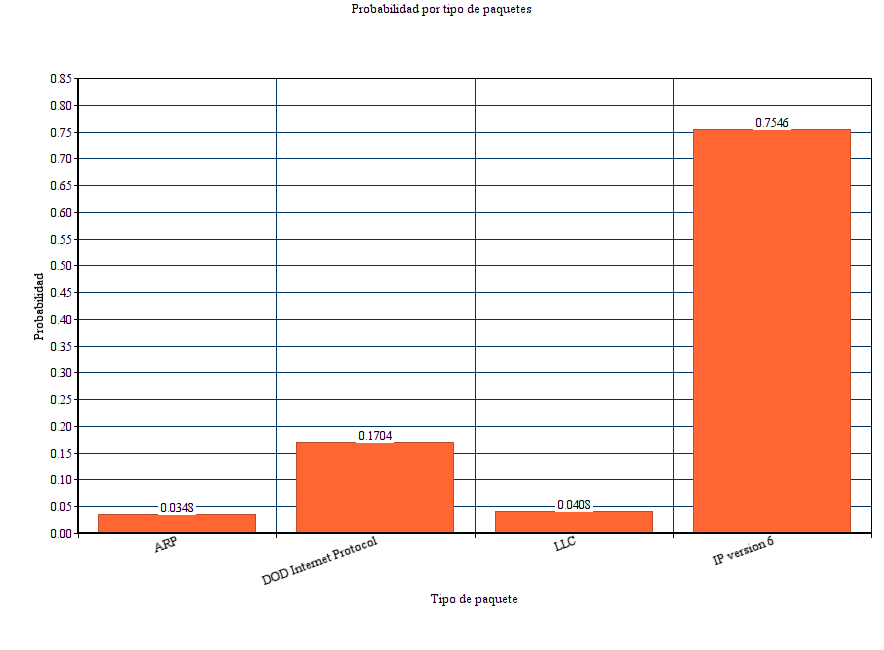
\includegraphics[width=0.7\textwidth]{exp4-graficos/exp4_1.png}
\end{center}

En la im\'agen se puede ver como la mayor\'ia de los paquetes capturados corresponden al tipo IP version 6, con un 75\%. Mientras que la probabilidad de los ARP es de aproximadamente 3\%. 
El protocolo IPv6 es una versión del protocolo IP que reemplaza a la antigua IPv4. Que haya una probabilidad tan alta de paquetes de este tipo muestra que en la red hay un alto uso de paquetes de datos. 
La entrop\'ia o incertidumbre observada del total de la fuente es 1.1 con lo cual se puede ver que es m\'as bien baja. Bas\'andonos en la teoro\'ia
de la informaci\'on podemos ver que la probabilidad de un s\'imbolo del tipo IP acapara la mayor\'ia de la fuente, logrando que uno pueda inferir que si uno toma un s\'imbolo emitido por la fuente este va a ser del tipo IP casi con seguridad.

Ahora vamos a referirnos estrictamente a los paquetes ARP. En total capturamos 11297 de ellos. Analizemos de qu\'e IP provienen: 

\begin{center}
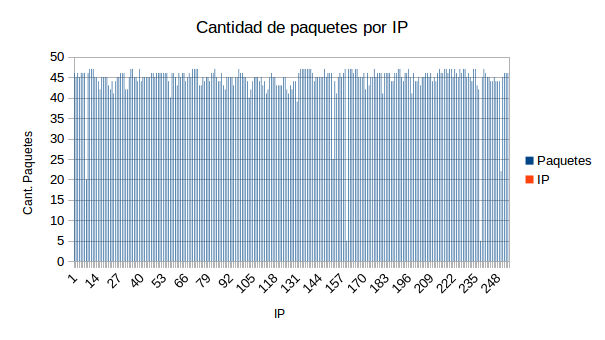
\includegraphics[width=0.7\textwidth]{exp4-graficos/exp4_2.png}
\end{center}


Estos resultados nos desconcertaron. En el gr\'afico se observan que los paquetes ARP se ditribuyen en las 255 IP que pertenecen a la red privada. La explicaci\'on que encontramos es que el protocolo que utiliza el router es DHCP (Dynamic Host Configuration Protocol). Este protocolo asigna IP a los dispositivos autom\'aticamente, y las intercambia din\'amicamente. La ventaja de este protocolo es la comodidad no tenemos que conocer los par\'ametros de la red, como rango de direcciones, m\'ascara de red o puerta de enlace. 

La entropía de los paquetes ARP es 7.97777628535, y esto se debe a que la mayoría de las IP tienen una probabilidad de aparecer muy parecida. Ya que se está cambiando constantemente de IP dinámica, todas las IP aparecen un número parecido de veces. Esto hace que el próximo paquete ARP que se capture se pueda predecir con bastante exactitud. 







